\documentclass[12pt]{article}
%%%%%%begin preamble
\usepackage[hmargin=1in, vmargin=1in]{geometry} % Margins
\usepackage{hyperref}
\usepackage{url}
\usepackage[numbers]{natbib}
\usepackage{graphicx}
\usepackage{amsmath}
\usepackage{amsfonts}
\usepackage{amssymb}
\usepackage{wrapfig}

\usepackage{multicol}
\usepackage{etoolbox}
%\patchcmd{\thebibliography}{\section*{\refname}}
%    {\begin{multicols}{2}[\section*{\refname}]}{}{}
%\patchcmd{\endthebibliography}{\endlist}{\endlist\end{multicols}}{}{}


\usepackage[normalem]{ulem}
\usepackage{xcolor}
\newcommand{\edit}[2]{\textcolor{purple}{\sout{#1} \textbf{#2}}}

\hypersetup{
  colorlinks   = true,
  %citecolor    = blue
  citecolor    = blue
  % gray is not being found!?!
  % gray is found if pdfpages is used... crap.
  %citecolor    = grey
  %citecolor    = Gray
}


%% headers
\usepackage{fancyhdr}
\pagestyle{fancy}
\fancyhf{} % sets both header and footer to nothing
\lhead{Evan H. Anders}
\rhead{Research Statement}
\cfoot{\footnotesize{\thepage}}
%\pagestyle{empty}
%\pagenumbering{gobble}
%\renewcommand*{\thefootnote}{\fnsymbol{footnote}}

\renewcommand{\vec}{\ensuremath{\boldsymbol}}
\newcommand{\dedalus}{\href{http://dedalus-project.org}{Dedalus}}
\newcommand{\del}{\ensuremath{\vec{\nabla}}}
\newcommand{\scrS}{\ensuremath{\mathcal{S}}}

\newcommand{\prf}{PRF}
\newcommand{\prr}{PRR}
\newcommand{\ssr}{SSR}
\newcommand{\araa}{ARAA}
\newcommand{\mnras}{MNRAS}
\newcommand{\aap}{A\&A}
\newcommand{\apjl}{ApJL}
\newcommand{\apj}{ApJ}
\newcommand{\apjs}{ApJL}

\newcommand{\sct}[1]{\vspace{0.3cm}\hspace{-\parindent}\textbf{\underline{#1}}\hspace{0.3cm}}

%\newcommand{\nosection}[1]{%
%  \refstepcounter{section}%
%  \addcontentsline{toc}{section}{\protect\numberline{\thesection}#1}%
%  \markright{#1}}
%\newcommand{\nosubsection}[1]{%
%  \refstepcounter{subsection}%
%  \addcontentsline{toc}{subsection}{\protect\numberline{\thesubsection}#1}%
%  \markright{#1}}

%\usepackage{atbegshi}
%%%%%%end preamble


%Make bibliography 2col
\bibliographystyle{apj_small}
\makeatletter
\renewenvironment{thebibliography}[1]
     {\begin{multicols}{2}[\paragraph*{\refname}\vspace{-0.1in}]%
      \@mkboth{\MakeUppercase\refname}{\MakeUppercase\refname}%
      \list{\@biblabel{\@arabic\c@enumiv}}%
           {\settowidth\labelwidth{\@biblabel{#1}}%
            \leftmargin\labelwidth
            \advance\leftmargin\labelsep
            \@openbib@code
            \usecounter{enumiv}%
            \let\p@enumiv\@empty
            \renewcommand\theenumiv{\@arabic\c@enumiv}}%
      \setlength{\itemsep}{-2pt}
      \sloppy
      \clubpenalty4000
      \@clubpenalty \clubpenalty
      \widowpenalty4000%
      \sfcode`\.\@m}
     {\def\@noitemerr
       {\@latex@warning{Empty `thebibliography' environment}}%
      \endlist\end{multicols}}
\makeatother



\begin{document}
\thispagestyle{fancy}

\sct{Context \& Aims}
Current and next-generation space- and ground-based observatories are revolutionizing precision observations in astrophysics.
%Lightcurves from \emph{Kepler} and \emph{TESS} \citep{ricker_etal_2016} have enabled the detection of thousands of planets \citep{huang_etal_2020}, and
%ESA's \emph{PLATO} will gather up to a million stellar lightcurves in search of Earth analogues \citep{montalto_etal_2021}.
%Spectroscopic follow-up observations will soon be sensitive enough to detect the radial velocity signal of Earth-like planets around Sun-like stars \citep[$\sim 10$ cm/s,][]{crass_etal_2021}.
%These datasets have fueled a rapid expansion of the field of asteroseismology, which can probe the radial dependence of mixing processes in stellar interiors \citep[][]{pedersen_etal_2021}.
%Mixing processes which bring fresh fuel into the stellar core affect subsequent stellar evolution and the mass of the eventual stellar remnant, so mixing uncertainties affect predictions of the populations of white dwarfs, neutron stars, and black holes.
%Kilometer-scale gravitational wave observatories (e.g., \emph{LIGO}/\emph{VIRGO} and soon \emph{Kamioka}) will continue to challenge models with new constraints on the populations of massive remnants \citep{abbott_etal_2018}.
%Proposed space-based gravitational-wave observatories (\emph{LISA}) will complement these observations with extreme sensitivity to the galactic white dwarf population \citep{robson_etal_2019}.
%
%
Discoveries ranging from exoplanets to black holes rely on high-precision stellar evolution models for calibration \citep{mesa6}, and convection introduces uncertainty into these models.
Mixing at the convective core boundary of massive stars ($M_* \gtrsim 1.1 M_\odot$) leads to core mass uncertainties of up to 70\% \citep{kaiser_etal_2020}, making the evolutionary pathway of a star from birth to death unclear.
Strange iron-opacity-driven convection in the outer layers of massive stars can also inflate the stellar surface and alter mass loss via winds at the stellar surface \citep{kohler_etal_2015}.
On lower mass stars, luminosity variations from surface convective can completely cover the signals of earth-like planets in radial velocity measurements \citep{crass_etal_2021}.
These processes and signals result from nonlinear 3D convection, which is poorly modeled in stellar evolution calculations and theoretical prescriptions.
%\textbf{Modern precision observations have revealed major theoretical shortcomings in models of convection and demand a new state-of-the-art set of convective simulations. }


%These observational puzzles demand models that go beyond the current state-of-the-art.
\textbf{My research group's goal will be to build a next-generation set of global and local 3D numerical simulations, which will answer the following three questions:}\vspace{-0.2cm}
\begin{enumerate}
    \item How large are convective cores in massive stars? \vspace{-0.2cm}
    \item How does iron-bump convection affect the stratification of massive stars, and how does this affect the color and luminosity of these stars?\vspace{-0.2cm}
    \item How does planet-obscuring convective blueshift vary across stellar mass?\vspace{-0.2cm}
\end{enumerate}

\sct{My Prior Research}
My research is rooted in fluid dynamics and inspired by observations of stars.
I use the \emph{Dedalus} \citep{burns_etal_2020} pseudospectral code to design and run state-of-the-art simulations which I use to learn about mixing processes like convection in stars.
\textbf{A core focus of my research has been to push the boundaries of \emph{time} evolution, while other studies have focused on \emph{spatial} resolution; my focus on the time domain has led to key discoveries in my career.}
When I was a graduate student, I focused on fundamental studies of convection.
I studied heat transport in compressible convection with  \citep{anders_etal_2019_rot} and without \citep{anders_brown_2017} rotation.
I studied how fast convection interacts with the slow evolution of the background thermal structure in convective regions \citep{anders_etal_2018,anders_etal_2020}.
I also studied convection at the smallest scales, examining individual downflows in the Sun's convection zone \cite{anders_etal_2019_thermals}.
As a postdoctoral fellow at Northwestern, I have connected my theoretical research with modern observational puzzles.
I have formed collaborations with observers and 1D modelers alike to understand what sets the position of a convective boundary \citep{anders_etal_2022b}, and I have discovered the process that inflates the convective cores of stars relative to standard models \citep{anders_etal_2022a}.
I am now finishing a project focusing on gravity wave generation by core convection and the observable signals of these waves, for direct comparison with e.g., asteroseismic observations.

\sct{Focus I: Convective Boundary Mixing}
Observations consistently demonstrate a need for improved models of convective boundary mixing (CBM) \citep{johnston2021}.
Stellar models require an unexplained mass-dependent CBM to reproduce observed eclipsing binary populations  \citep{claret_torres_2019}.
The amount of CBM used in stellar evolution models modifies how a star's luminosity and effective temperature evolve \citep{castro_etal_2014,higgins_vink_2019}.
Asteroseismology now allows us to directly probe near-core CBM, revealing extensive mixing occurs near convective core boundaries \citep{michielsen_etal_2019, pedersen_etal_2021}.

To understand the fluid dynamical picture behind CBM, my group will create simulations of the cores of massive stars using the \emph{Dedalus} \citep{burns_etal_2020} code.
These simulations will differ from past simulations of massive stars, because they will include the full ``ball'' geometry of the convective core, they will employ the fully compressible equations without any luminosity boosting, and they will be relaxed into thermal equilibrium (See Fig.~\ref{fig:star} or \url{https://vimeo.com/483598178} for a preliminary example of one of these simulations).
\emph{Dedalus} was recently updated with the state-of-the-art ability to simulate flows that pass through the coordinate singularity at $r = 0$ in spherical coordinates \citep{vasil_etal_2019,lecoanet_etal_2019}; most prior codes used a spherical shell geometry with a small interior ``cutout'' of the core.
Our implicit-explicit (IMEX) timestepping scheme allows us to circumvent timestepping restrictions from fast sound waves \citep{anders_brown_2017}, so we can take fast timesteps without boosting the luminosity as many prior simulations have done.
Evolving a simulation to thermal equilibration using classic timestepping techniques can take thousands of convective overturn timescales \citep{anders_etal_2022a,anders_etal_2022b}.
Fortunately, I have developed methods of ``accelerated evolution'' \citep{anders_etal_2018}, which self-consistently equilibrate simulations using an order of magnitude fewer cpu-hours than traditional timestepping.

My group will study CBM in fully compressible simulations whose background stratifications are based upon MESA (Modules for Experiments in Stellar Astrophysics) models of massive stars.
We will study non-rotating and rotating stars with masses varying in the range $M_* = 1.1-40 M_{\odot}$ (the lowest masses where convective cores appear, up to high masses).
Our results will inform a 1D implementation of convective boundary mixing, which we will then implement into the open-source MESA software instrument.
Throughout this process, I will build our simulation code with ease-of-use for the user in mind, and this code will be made publicly available and citeable so that the community has access to a robust tool for studying stellar fluid dynamics.

\begin{wrapfigure}{r}{0.5\textwidth}
  \begin{center}
      \vspace{-1.6cm}
    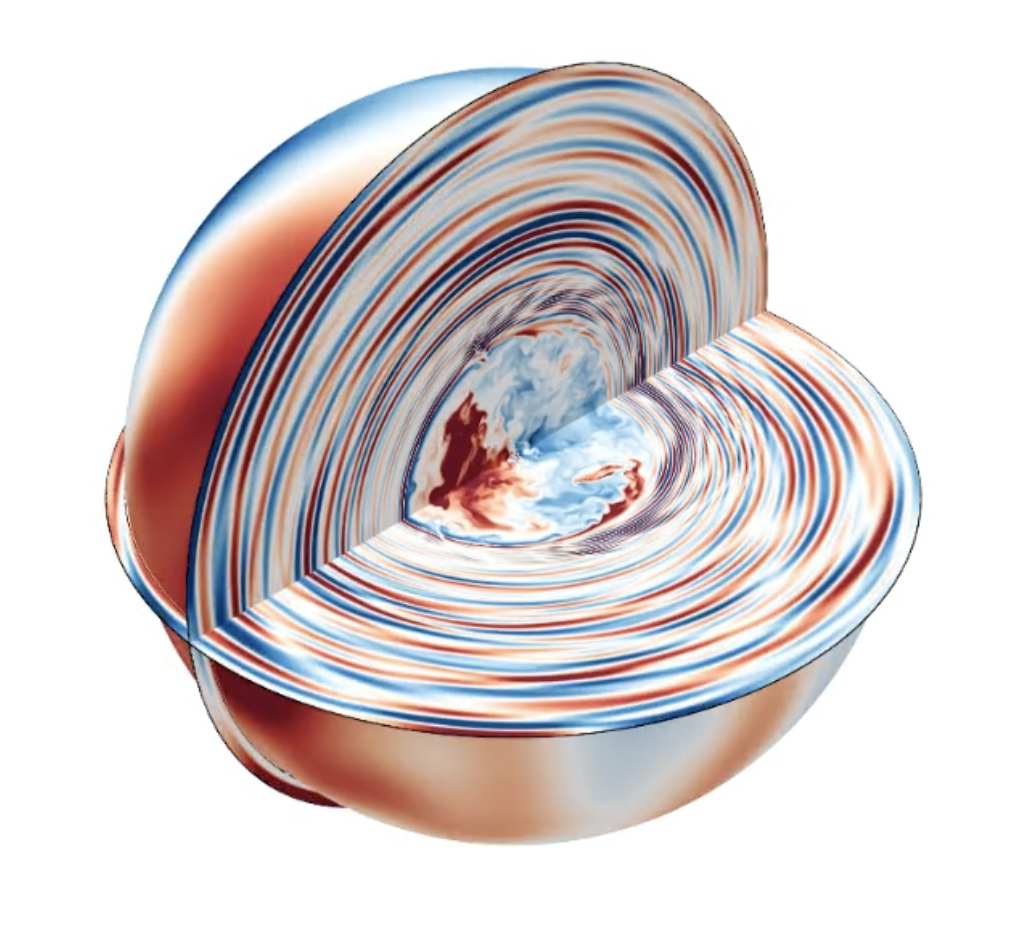
\includegraphics[width=0.45\textwidth]{dedalus_massive_star.png}
      \vspace{-1.3cm}
  \end{center}
    \caption{A simulation I ran in \emph{Dedalus} of a {$40 \,M_{\odot}$} star. 
    The entropy field is visualized; red is hot and buoyantly rises, blue is cold and falls. 
    We see a convective core with a strong dipole flow and an outer radiative envelope with internal gravity waves. \label{fig:star}}
    \vspace{-0.5cm}
\end{wrapfigure}
I will study CBM in fully compressible simulations whose background stratifications are based upon \emph{MESA} (Modules for Experiments in Stellar Astrophysics) models of massive stars.
I will study non-rotating and rotating stars with masses varying in the range $M_* = 1.1-40 M_{\odot}$ (the lowest masses where convective cores appear, up to high masses).
My results will calibrate a 1D implementation of convective boundary mixing, which I will then implement into the open-source \emph{MESA} software instrument.
Throughout this process, I will build my \emph{Dedalus} simulation code with ease-of-use for the user in mind, and this code will be made publicly available and citeable so that the community has access to a robust tool for studying fluid dynamics in massive stars.


\textbf{\underline{\emph{Deliverable:}} The first rotating, 3D simulations of core convection that include $\boldsymbol{r = 0}$ and reach thermal equilibrium.}

\textbf{\underline{\emph{Student Opportunities:}}} Advanced undergraduate students will have opportunities to study 1D stellar evolution models with convective boundary mixing.
A graduate thesis could consist of running many 3D simulations, generating the parameterization of CBM, and implementing it into MESA (three separate papers).
Core convection generates asteroseismically-observable waves, and the generation and propagation of these waves is poorly modeled in simulations and could be the focus of a graduate thesis.

\sct{Focus II: Optically thick, low-efficiency Iron-Bump Convection.}
In addition to vigorous core convection, it is now accepted that massive stars have opacity-driven convective shells in their envelopes \citep{cantiello_etal_2009}.
For stars with masses $\gtrsim 8 M_{\odot}$, an ``Iron-Bump Convection Zone'' (FeCZ) appears as a result of the opacity of iron.
These convection zones are odd: they approach the Eddington luminosity limit, are very thin, and exhibit high-Mach number, turbulent flows \citep{jermyn_etal_2022_atlas}.
%However, unlike the convection zones at the surface of lower-mass stars (e.g., the Sun), these convection zones generally appear at high optical depths \citep[fig 59 of][]{jermyn_etal_2022_atlas}.
This odd convection has not been studied in detail, but the presence of these convection zones influences the stellar structure and evolution appreciably \citep{kohler_etal_2015}.


Numerical simulations of these convection zones are extremely limited.
Those simulations which have been performed \citep{jiang_etal_2015, schultz_etal_2020} demonstrate interesting dynamics and thermodynamics.
The high-Mach number convection supports a large dynamic pressure, which can inflate the star.
I will use \emph{Dedalus} to build on the high-Mach number, fully compressible simulations that I studied in Ref.~\citep{anders_brown_2017} by including iron bump opacity effects.
My research group will study a span of simulations varying stellar mass from $8-60 M_{\odot}$ and at various stellar ages to understand the turbulent pressure component that arises from these zones.

We will study iron bump convection in Cartesian, optically thick models \citep[good approximations,][]{jermyn_etal_2022_atlas}.
We will measure how the turbulent pressure modifies the background pressure, incorporate this into MESA, then study the observable consequences of this pressure.

\textbf{\underline{\emph{Deliverable:}} The first 3D simulations of FeCZs at many stellar masses.}

\textbf{\underline{\emph{Student Opportunities:}}} Advanced undergraduate students will study how FeCZs change surface observables of stars using current prescriptions, and examine evolutionary (wind loss) consequences in detail.
A graduate thesis could consist of modifying \emph{Dedalus} to include iron bump opacity, a simulation suite, and incorporating the dynamical pressure into MESA.

\sct{Focus III: Convective Blueshift}
An Earth-like planet around a Sun-like star produces a radial velocity (RV) signal on the order of 10 cm/s.
Extreme Precision RV (EPRV) instruments are now sensitive enough to observe signals below this threshold, but stellar surface convection produces RV signals much larger than 10 cm/s \citep{crass_etal_2021}.
``Convective Blueshift" (CBS) is a net blueshifting of spectral line wings resulting from the convection granulation pattern (warm upflows cover more surface area than cold downflows).
CBS measurements were recently obtained for hundreds of stars \citep{liebing_etal_2021}; a tight cubic relationship is found between the effective temperature and CBS, which may result from the changing size of convective granules. %careful about "robust"
In order to robustly remove CBS from EPRV signals, empirical fits must be tested and validated against theory and nonlinear convection simulations. 

Convection at the Sun's surface has been studied in exquisite detail in Cartesian simulations which include full radiative transfer (RT) treatments \citep[e.g.,][]{rempel2020, danilovic_etal_2022}.
Unfortunately this full RT treatment makes these simulations costly, so studying CBS for many different stars is unfeasible.
My research group will develop simulations with efficient, reduced models of RT to create a simulation suite spanning the lower main sequence and create synthesized observables to compare with existing CBS datasets.

I will lead efforts to create fully compressible convection simulations in \emph{Dedalus}.
My group will implement convection under the Eddington tensor approximation \citep[e.g., ref.][sct.~XI.G]{burns_etal_2020}, under a grey atmosphere approximation with a ``realistic'' radiative diffusivity \citep{barekat_brandenburg_2014}, and under a simplified diffusion approximation with an idealized radiative diffusivity and an imposed surface cooling.
Fundamental properties of interest are the size and flow speed of convective granules.
From these simulations, we will synthesize observables of CBS which can be compared to observations \citep{liebing_etal_2021}.

\textbf{\underline{\emph{Deliverable:}} The first simulated constraint from 3D simulations on convective blueshift spanning the lower main sequence.}

\textbf{\underline{\emph{Student Opportunities:}}} Advanced undergraduate students could write a paper gaining an understanding of the fluid parameter space that is probed by the convection zones at the surfaces of these stars.
A graduate student could easily make this work the focus of a PhD thesis.
Developing and studying the radiative-convective simulations is a well-posed task which could produce multiple papers.
The span of simulations which studies stars along the main sequence is another paper which offers the student an opportunity to connect to the (larger) community of astrophysical observers in a field (exoplanetary science) which is currently very well-funded.


\sct{Open Science and Outreach}
Open science is very improtant to me; my group will employ best-coding-practices and upload our simulation code and run scripts to GitHub and Zenodo so that our science can be easily reproduced.
I am interested in finding ways to communicate with the general public about my research in addition to about astronomy and astrophysics broadly.
My simulations provide many avenues for creating appealing visualizations that can help us connect to the public, and I am interested in exploring ways of presenting our results to the differently-abled, such as through sonification of wave spectra or turbulent spectra that our convection produces.

{\scriptsize
\bibliography{biblio}
}
\end{document}
